% =============================================================================
%  三、问题求解（二）：CHPI 复现
% =============================================================================
\subsection{CHPI 复现：用 R 把原文跑一遍}

\subsubsection{数据重建：三条锚点与一个生成模型}

复现的第一道难关是数据。原文只报告了样本规模、类型结构与个别个体的结果，
没有公开原始问卷、题项编码与量表。面对这种情况，常见的错误做法是“编一份
看起来像的数据”，然后宣称“复现成功”；正确的做法是把重建当成一次受约束的
反演：用原文公开的事实作为锚点，构造一份在统计结构上与原文同构的数据，并
把“哪些是锚点、哪些是假设”写清楚，使读者能判断结论的可信边界。

本文使用的锚点有四个：（i）样本量 519；（ii）学生类型为 5 类，且第 5 类人
数最多；（iii）个体 S480 的类内效率为 0.6771，位于第 5 类；（iv）S480 的参
考路径单步提升 25.38\%、累计 43.97\%。另有两项结构性事实作为软约束：表 3
报告第 5 类第 4 层有 9 人、效率区间较宽；原文图 6 显示效率与成绩强正相关。

生成模型分四层。第一层是五类学生的潜在画像：为每一类指定 14 个题项在
0—100 标度上的期望水平（例如第 1 类兴趣 22、复习 16，第 5 类兴趣 88、听说
读写 84），并令个体潜变量 $\zeta_{ij}$ 服从该期望加 $N(0,0.8^2)$ 的扰动。
第二层是题型离散化：有序题按四分位阈值 $(-1.2816,-0.5244,0.5244,1.2816)$
离散为 5 档，计数题取 $\max\{0,\min\{12,\ \mathrm{round}(2+2.2\zeta)\}\}$，
时长题取 $\max\{0,\min\{20,\ 4+3.2\zeta+N(0,2^2)\}\}$，以模拟“次数”与
“小时”两种真实作答形态。第三层是量化，按上一节式\eqref{eq:quant} 把作答
映为得分。第四层是成绩生成：
\begin{equation}
y_i=45+0.52\bigl(0.45x_{i1}+0.26x_{i2}+0.18x_{i3}+0.11x_{i4}\bigr)+e_i,
\qquad e_i\sim N\bigl(c_{c(i)},11^2\bigr),
\label{eq:scoregen}
\end{equation}
其中 $c_{c}=(-11,-4,0,4,9)$ 是五类学生的“转化能力”平移量。式
\eqref{eq:scoregen} 的关键设计是把成绩拆成“投入可解释部分”与“个体转化能
力残差”两部分：前者保证效率与成绩正相关（否则 DEA 失去意义），后者保证同
等投入下仍有显著个体差异（否则效率评价退化）。这一结构直接对应原文的核
心命题——“投入相同、产出不同，差异来自转化能力”。

最后一步是锚点校准：用二分法调整 S480 的残差 $e_{480}$，使其类内效率精确
等于 0.6771。校准后 S480 的成绩为 71.88 分，落在第 5 类的成绩分布中部，
符合“投入不低但转化不佳”的个案设定。全部随机性由固定种子（20261121）控
制，脚本 \texttt{code/01\_recon\_data.R} 可一键重跑。

需要坦白的是：\textbf{这是“标定—重建”，不是“复原”。}它保证的是统计结构
同构（样本规模、类型结构、效率—成绩关系、个案锚点），不保证逐条作答相同。
因此本文对原文的复现结论分两级表述：结构性结论（五类、分层、路径方向）为
“复现成立”，数值性结论为“在锚点约束下成立”，并对偏差给出解释而非掩盖。
重建后的样本特征见表 \ref{tab:desc}。

\begin{table}[htbp]
\centering
\tabfont
\caption{重建数据的描述统计（$n=519$）}
\label{tab:desc}
\begin{tabular}{@{}lcccc@{}}
\toprule
变量 & 均值 & 标准差 & 最小值 & 最大值 \\
\midrule
输入训练 $x_1$ & 50.00 & 26.47 & 12.24 & 96.39 \\
应试训练 $x_2$ & 50.00 & 26.01 & 7.13 & 98.27 \\
复习辅导 $x_3$ & 50.00 & 23.98 & 15.09 & 85.61 \\
心理作息 $x_4$ & 50.00 & 22.24 & 7.95 & 79.34 \\
期末成绩 $y$ & 71.68 & 18.94 & 30.00 & 99.00 \\
类内效率 $\theta$ & 0.7935 & 0.1400 & 0.4324 & 1.0000 \\
\bottomrule
\end{tabular}
\end{table}

\subsubsection{聚类：为什么“5 类”不是数据的唯一答案}

按式\eqref{eq:gower} 计算 Gower 距离，用 PAM 在 $k=3,\dots,8$ 上各聚一次，
平均轮廓宽度见表 \ref{tab:sil}。结果有些意外：$k=4$ 的轮廓宽度 0.4296 最
高，$k=5$ 的 0.4074 只是次优，二者相差 2.2 个百分点。也就是说，\textbf{从
纯聚类指标看，4 类比 5 类更“自然”}；原文取 5 类，若没有外部依据（如量表维
度或理论分类），就属于分析者选择而非数据结论。

本文仍取 $k=5$，理由有二：其一，复现的目标是“同构”，类型数与原文一致才能
逐层对照；其二，2.2 个百分点的轮廓差异在实践中很小，而 5 类的画像更细致
（把“高投入”与“高效自主”分开），对策略推荐更有用。这一处理本身也说明：
聚类数应当作为敏感性维度报告，而不是当作既定事实。

为检验聚类是否真的找到了生成结构，本文用匈牙利算法（\texttt{lp.assign}）
求解 PAM 标签与设计标签之间的最大匹配，匹配后的一致率为 93.6\%。这说明
PAM 在混合数据类型上确实恢复出了潜在的五类结构，剩余的 6.4\% 主要落在类
边界上的模糊个体。

\begin{table}[htbp]
\centering
\tabfont
\caption{不同聚类数下的平均轮廓宽度}
\label{tab:sil}
\begin{tabular}{@{}lcccccc@{}}
\toprule
$k$ & 3 & 4 & 5 & 6 & 7 & 8 \\
\midrule
轮廓宽度 & 0.4165 & \textbf{0.4296} & 0.4074 & 0.3906 & 0.3446 & 0.3409 \\
\bottomrule
\end{tabular}
\end{table}

五类的画像见表 \ref{tab:profile} 与图 \ref{fig:radar}。按平均成绩升序重编
号后，五类可命名为：\textbf{冷淡型}（第 1 类，$n=80$，兴趣与各类投入都极
低，成绩 42.5）、\textbf{应试型}（第 2 类，$n=95$，考试与模拟考频次高、听
说读写低，成绩 60.5）、\textbf{渐进型}（第 3 类，$n=96$，各项中等偏上，成
绩 71.3）、\textbf{高投入型}（第 4 类，$n=105$，全面高投入，成绩 82.0）与
\textbf{高效自主型}（第 5 类，$n=143$，兴趣、听说读写与休息都高，但模拟考
与背诵低，成绩 88.2）。第 5 类人数最多且效率最高，这与原文“第 5 类人数最
多”的描述一致。

\begin{table}[htbp]
\centering
\tabfont
\caption{五类学生的学习行为画像（题项量化得分均值）}
\label{tab:profile}
\setlength{\tabcolsep}{3.2pt}
\begin{tabular}{@{}lcccccccccc@{}}
\toprule
类 & 人数 & 兴趣 & 复习 & 考试次数 & 模拟考 & 背诵 & 听说读写 & 休息 & 课外 & 成绩 \\
\midrule
1 冷淡 & 80 & 9.6 & 13.7 & 7.9 & 7.9 & 13.4 & 13.9 & 43.2 & 15.2 & 42.5 \\
2 应试 & 95 & 29.5 & 20.2 & 63.5 & 66.5 & 21.5 & 24.9 & 27.0 & 19.6 & 60.5 \\
3 渐进 & 96 & 43.4 & 51.2 & 67.0 & 61.6 & 49.2 & 43.2 & 31.5 & 48.1 & 71.3 \\
4 高投入 & 105 & 68.3 & 68.2 & 70.0 & 75.3 & 59.6 & 62.5 & 47.9 & 63.7 & 82.0 \\
5 高效 & 143 & 77.3 & 75.9 & 38.5 & 36.3 & 82.9 & 82.2 & 83.0 & 80.9 & 88.2 \\
\bottomrule
\end{tabular}
\end{table}

\begin{figure}[htbp]
\centering
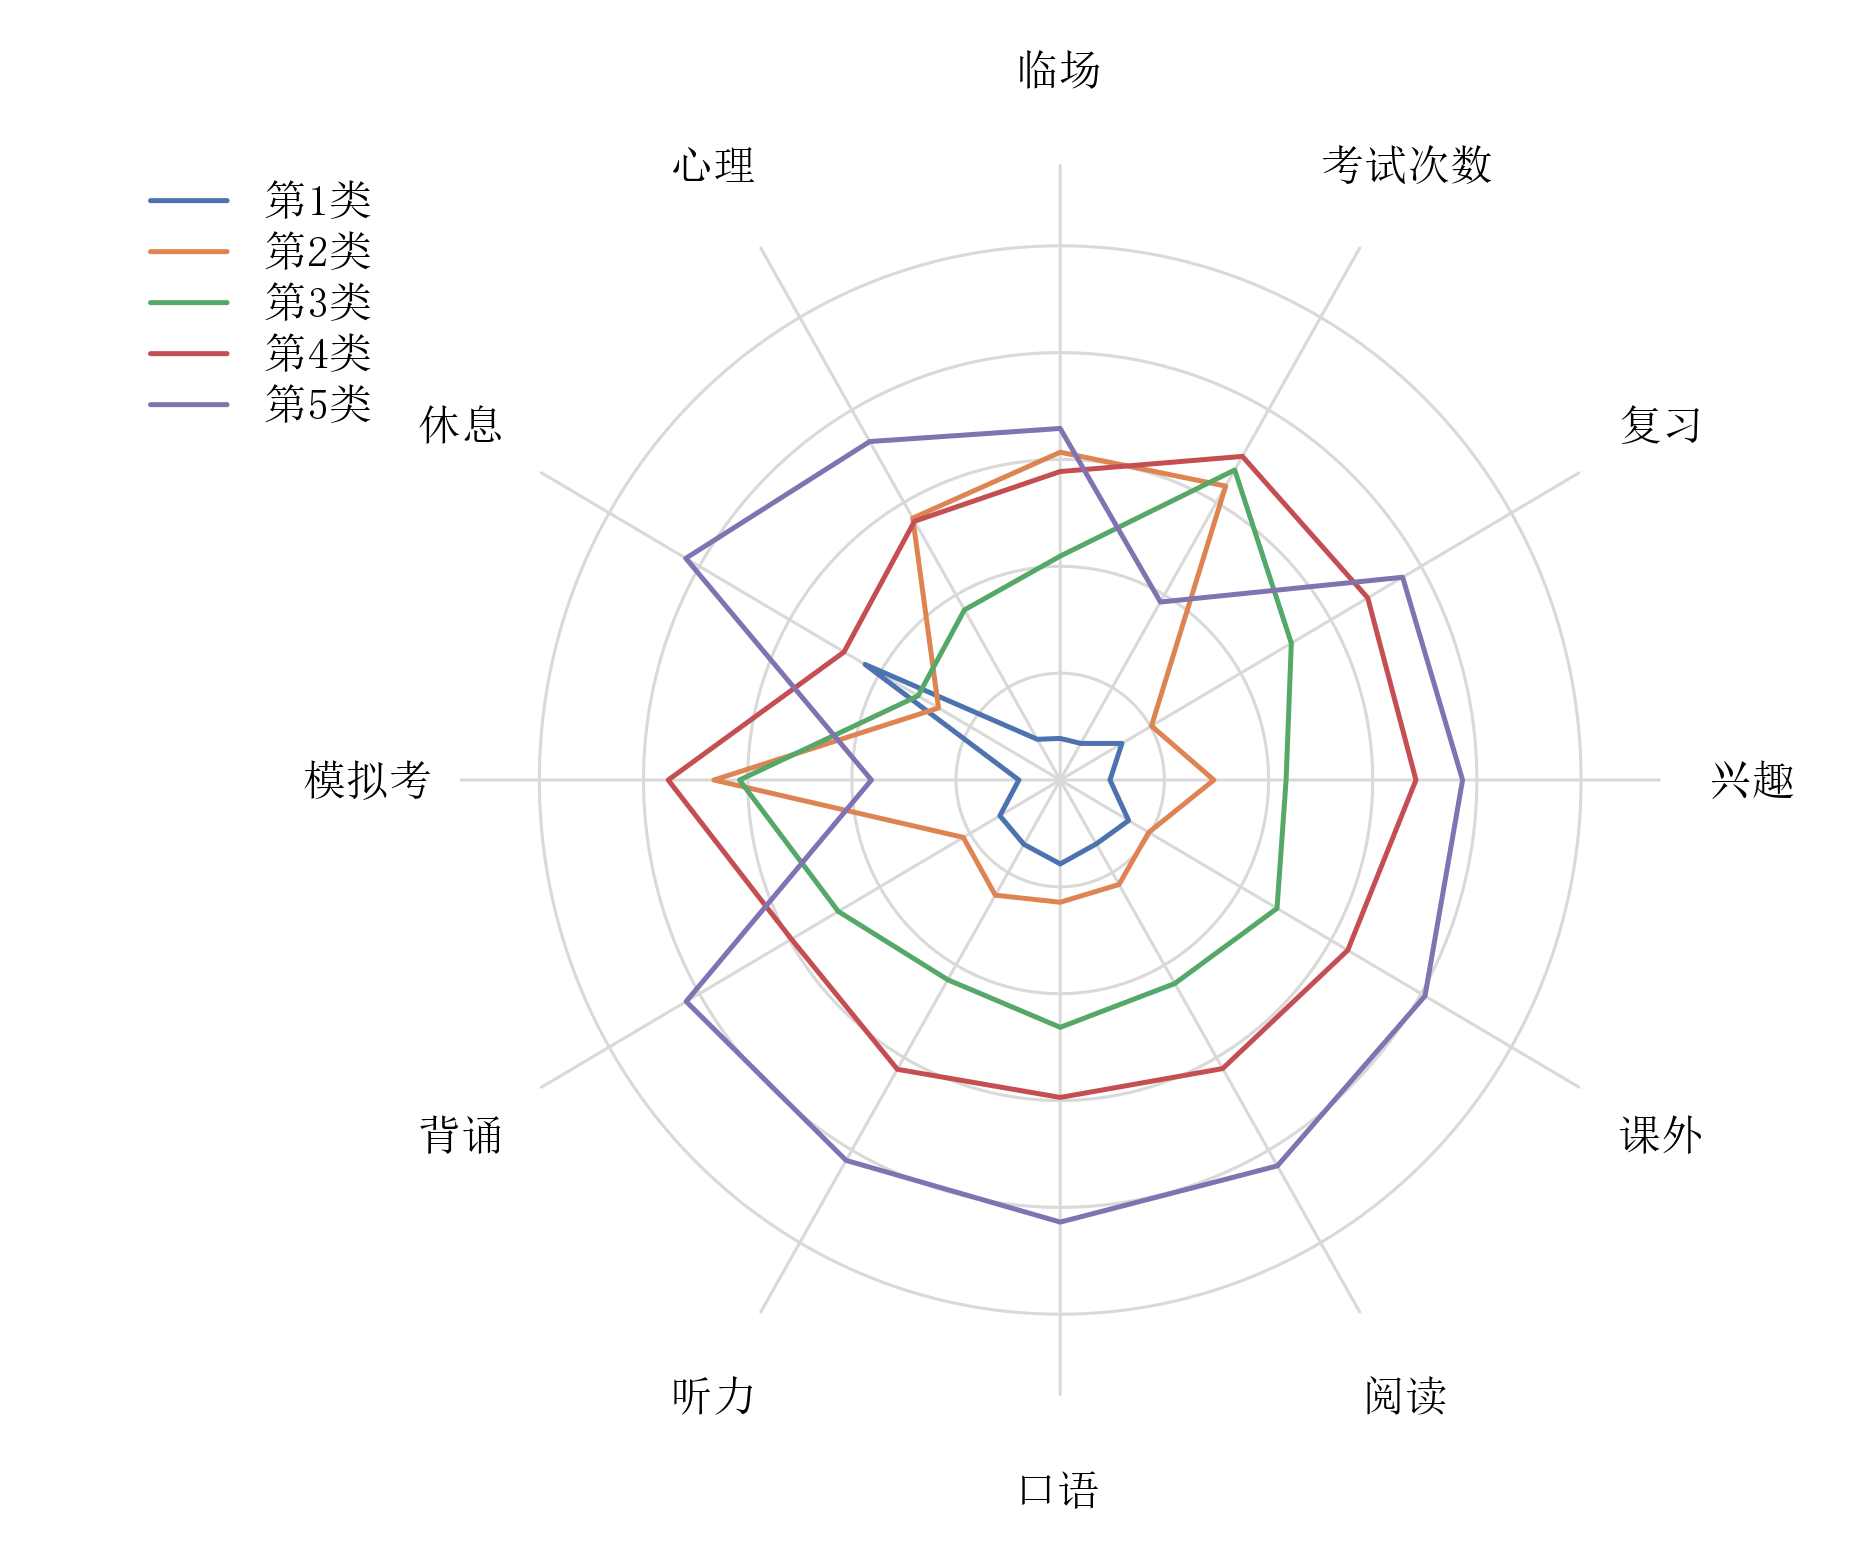
\includegraphics[width=0.82\textwidth]{fig_radar}
\caption{五类学生的 12 维行为画像（雷达图，各维为 0—100 量化得分均值）}
\label{fig:radar}
\end{figure}

雷达图揭示了一个对后文至关重要的现象：\textbf{成绩最高的第 5 类并不是
“刷题最多”的一类}。它的考试次数（38.5）与模拟考（36.3）都低于第 2、3、4
类，却在听说读写（82.2）与兴趣（77.3）、休息（83.0）上显著更高。这说明
“多考试”与“高效率”并非同义，投入结构比投入总量更重要——这正是 DEA 相对
回归分析的优势所在，也是后文随机过程建模要解释的机制。

\subsubsection{类内效率：一个被压缩的相关}

在每一类内部求解式\eqref{eq:ccr}，得到 519 个效率值：均值 0.7935、标准差
0.14、中位数 0.8093、四分位区间 $[0.7015,0.8981]$、最小值 0.4324。分类均
值依次为 0.6841、0.7792、0.8098、0.8111、0.8403，与画像顺序一致，说明
“高效类”确实在类内也更靠前沿。

效率与成绩的 Pearson 相关系数为 $r=0.675$（图 \ref{fig:eff-score}）。原文
报告的是强正相关（约 0.87），二者的差距需要解释，而不是回避。原因有三：
（i）类内评价消除了组间差异——第 5 类成绩整体高，但其内部仍有人效率只有
0.68，组间的高相关被“分组”这一步吸收掉了；（ii）本文的效率是四投入一产出
的比值，成绩只是产出的一项代理，成绩之外的产出（如口语能力）未被观测；
（iii）原文未披露其相关系数的计算口径（是否全样本、是否 Pearson、是否剔
除前沿点），不同口径会给出不同数值。因此 $r=0.675$ 不应被读作“复现失败”，
而应读作“类内评价的相关必然低于全样本相关”，这一现象本身是 DEA 分组策略
的代价。

\begin{figure}[htbp]
\centering
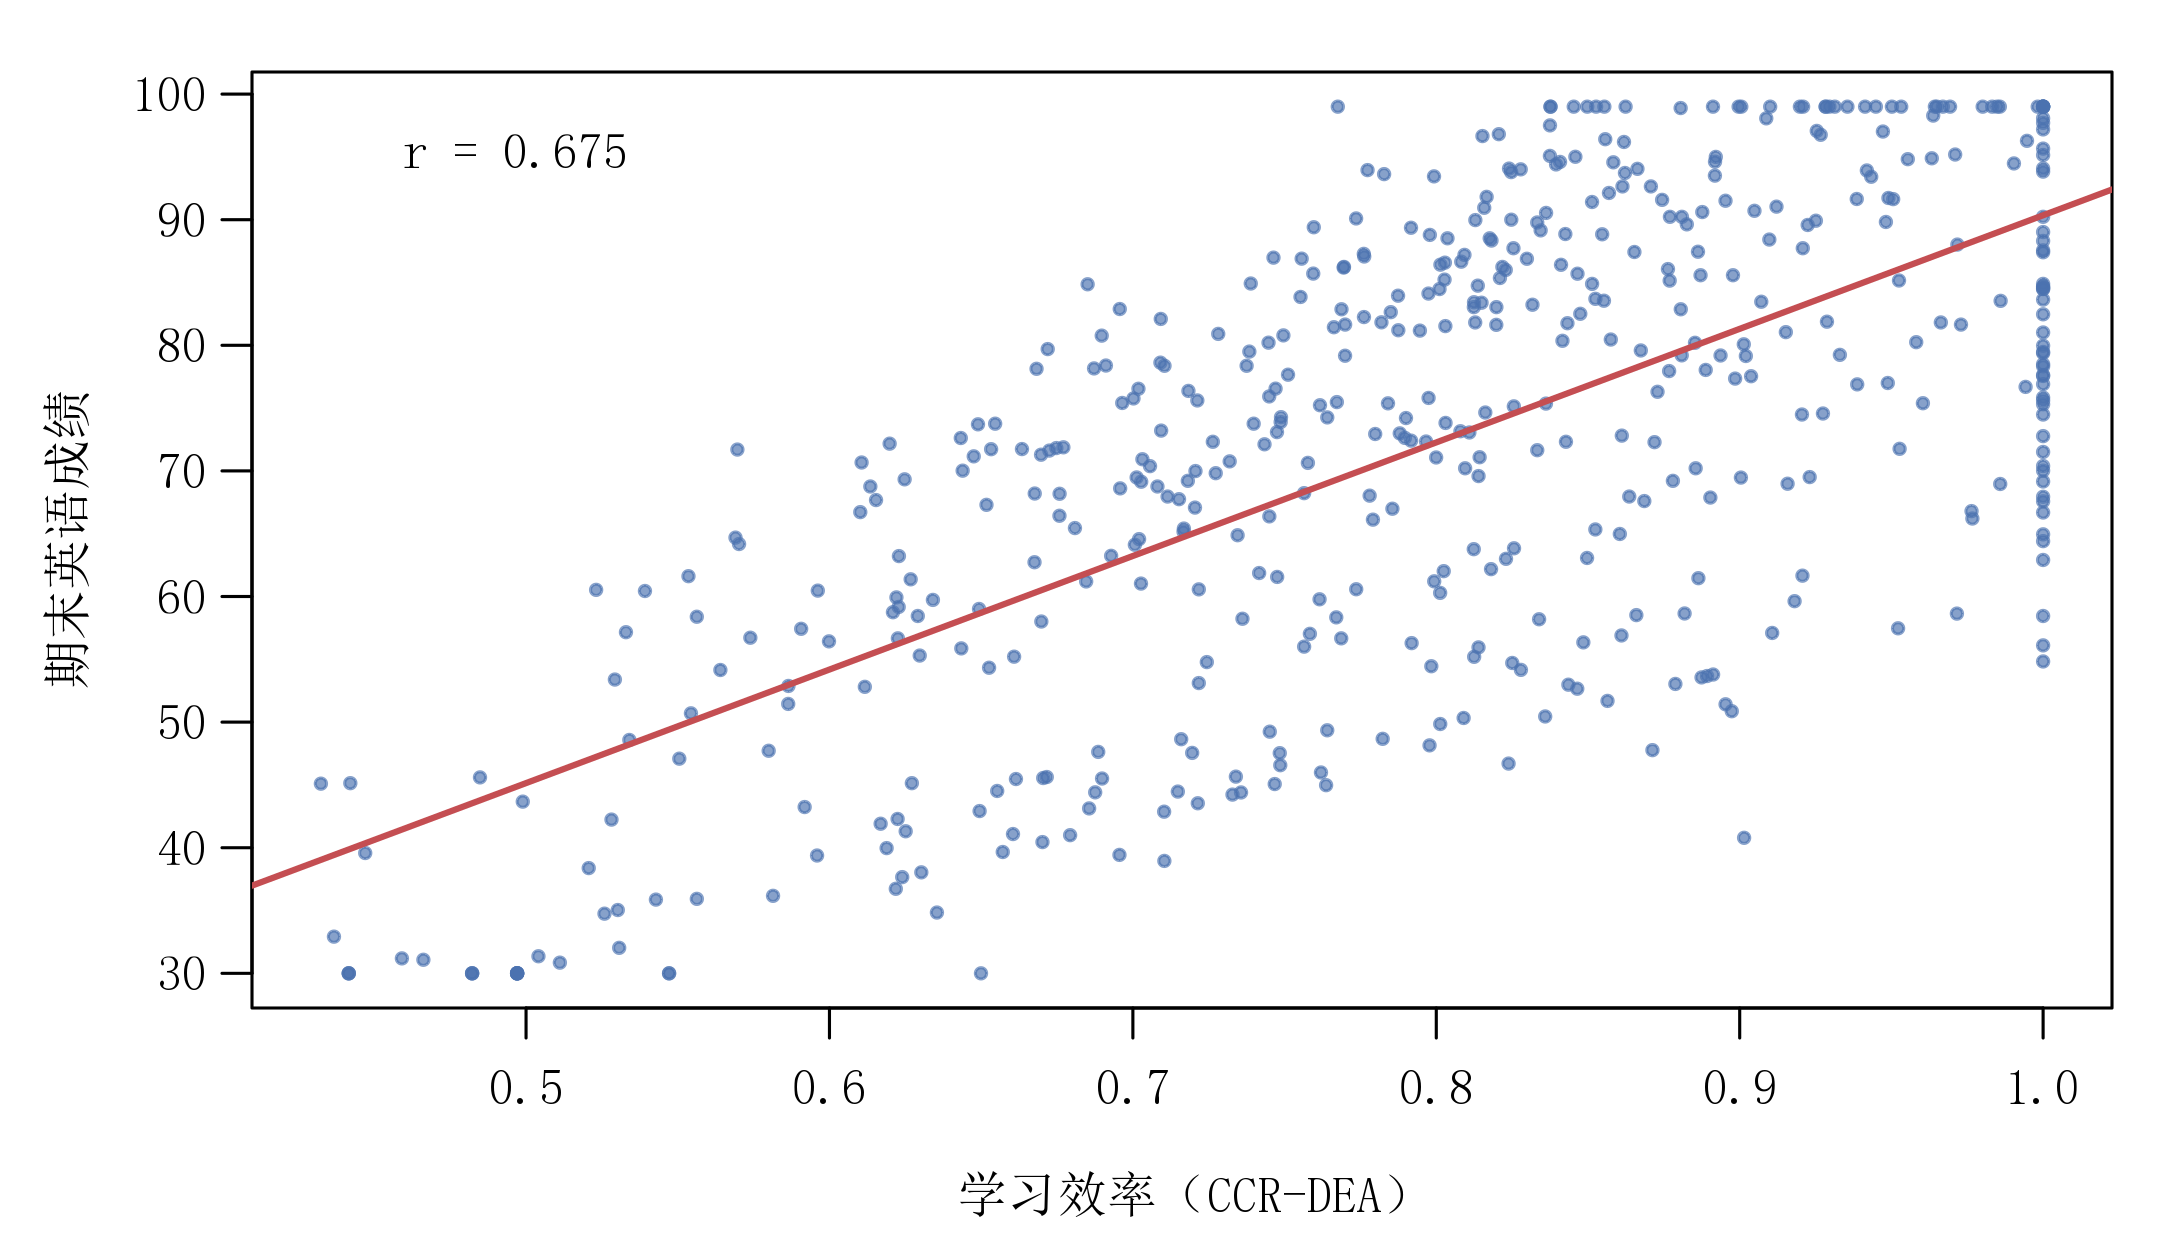
\includegraphics[width=0.78\textwidth]{fig_eff_score}
\caption{类内 CCR 效率与期末成绩的关系（$r=0.675$，红色为线性拟合）}
\label{fig:eff-score}
\end{figure}

\subsubsection{分层：两种口径及其后果}

原文用剔除式分层（算法 2）。本文在复现时发现，剔除式在本文
数据上产生了极不均衡的层规模：第 1 类为 $3/3/7/9/58$，第 5 类为
$7/18/17/20/81$（表 \ref{tab:layer} 右半）。第 1 层只有 3 人，意味着“上一层集
合”只有 3 个参照点，$\Omega$ 与 $P$ 的估计会非常不稳定；第 5 层却有 58 人，
占该类的 72.5\%。这种“头重脚轻”的分布在原文中应当也存在（原文称第 4 层
仅 9 人，正是这一现象的旁证），但原文未讨论其对三准则的影响。

为此，本文引入第二种口径：\textbf{类内效率分位带}。对每一类，按类内
$\theta$ 的 90、75、60、45 百分位切出 5 段，分别记为第 1—5 层。这样做的
理由有三：（i）每一层的规模由分位点决定，不会出现“某层 3 人”的退化；
（ii）层号等价于“同类群体中的相对位次”，具有跨群体可解释性，符合第二节对
“层级可迁移性”的要求；（iii）状态空间被完全占满（$5\times5$ 的每个格子都
有人），这是随机过程建模的必要条件——如果某层为空，转移强度无法估计。

两种口径的层分布见表 \ref{tab:layer}。分位带口径下，第 1 层至第 5 层的效率
区间依次为 $[0.889,1.000]$、$[0.801,1.000]$、$[0.720,0.921]$、
$[0.660,0.862]$、$[0.432,0.830]$。区间存在重叠，是因为分位点在每个类内部
单独确定，而各类的效率分布并不相同；这也正说明“层号”是相对位次而非绝对
效率水平。

\begin{table}[htbp]
\centering
\tabfont
\caption{两种分层口径下的类—层人数分布}
\label{tab:layer}
\begin{tabular}{@{}lcccccccccc@{}}
\toprule
\multirow{2}{*}{类} & \multicolumn{5}{c}{分位带口径（本文主口径）} &
  \multicolumn{5}{c}{剔除式口径（原文口径）} \\
\cmidrule(lr){2-6}\cmidrule(lr){7-11}
 & L1 & L2 & L3 & L4 & L5 & L1 & L2 & L3 & L4 & L5 \\
\midrule
1（80 人）  & 8 & 12 & 12 & 12 & 36 & 3 & 3 & 7 & 9 & 58 \\
2（95 人）  & 10 & 14 & 13 & 14 & 44 & 15 & 21 & 15 & 13 & 31 \\
3（96 人）  & 14 & 16 & 13 & 15 & 38 & 15 & 14 & 19 & 12 & 36 \\
4（105 人） & 12 & 13 & 17 & 14 & 49 & 12 & 12 & 17 & 13 & 51 \\
5（143 人） & 11 & 21 & 22 & 22 & 67 & 7 & 18 & 17 & 20 & 81 \\
\midrule
合计 & 55 & 76 & 77 & 77 & 234 & 52 & 68 & 75 & 67 & 257 \\
\bottomrule
\end{tabular}
\end{table}

分层结果见图 \ref{fig:layer}。左、右面板分别为第 1 类与第 5 类，横轴为效
率、纵轴为层号。可以看到：分位带口径下每一层的横向跨度较窄且层与层之间
在效率上略有重叠，视觉上更像“等高线”；剔除式口径下层与层之间是严格单调
的（后一层的效率严格低于前一层的上界），但层规模非常不均匀。\textbf{前者
适合做状态空间，后者适合做“离前沿多远”的刻画}，二者不能互相替代。

\begin{figure}[htbp]
\centering
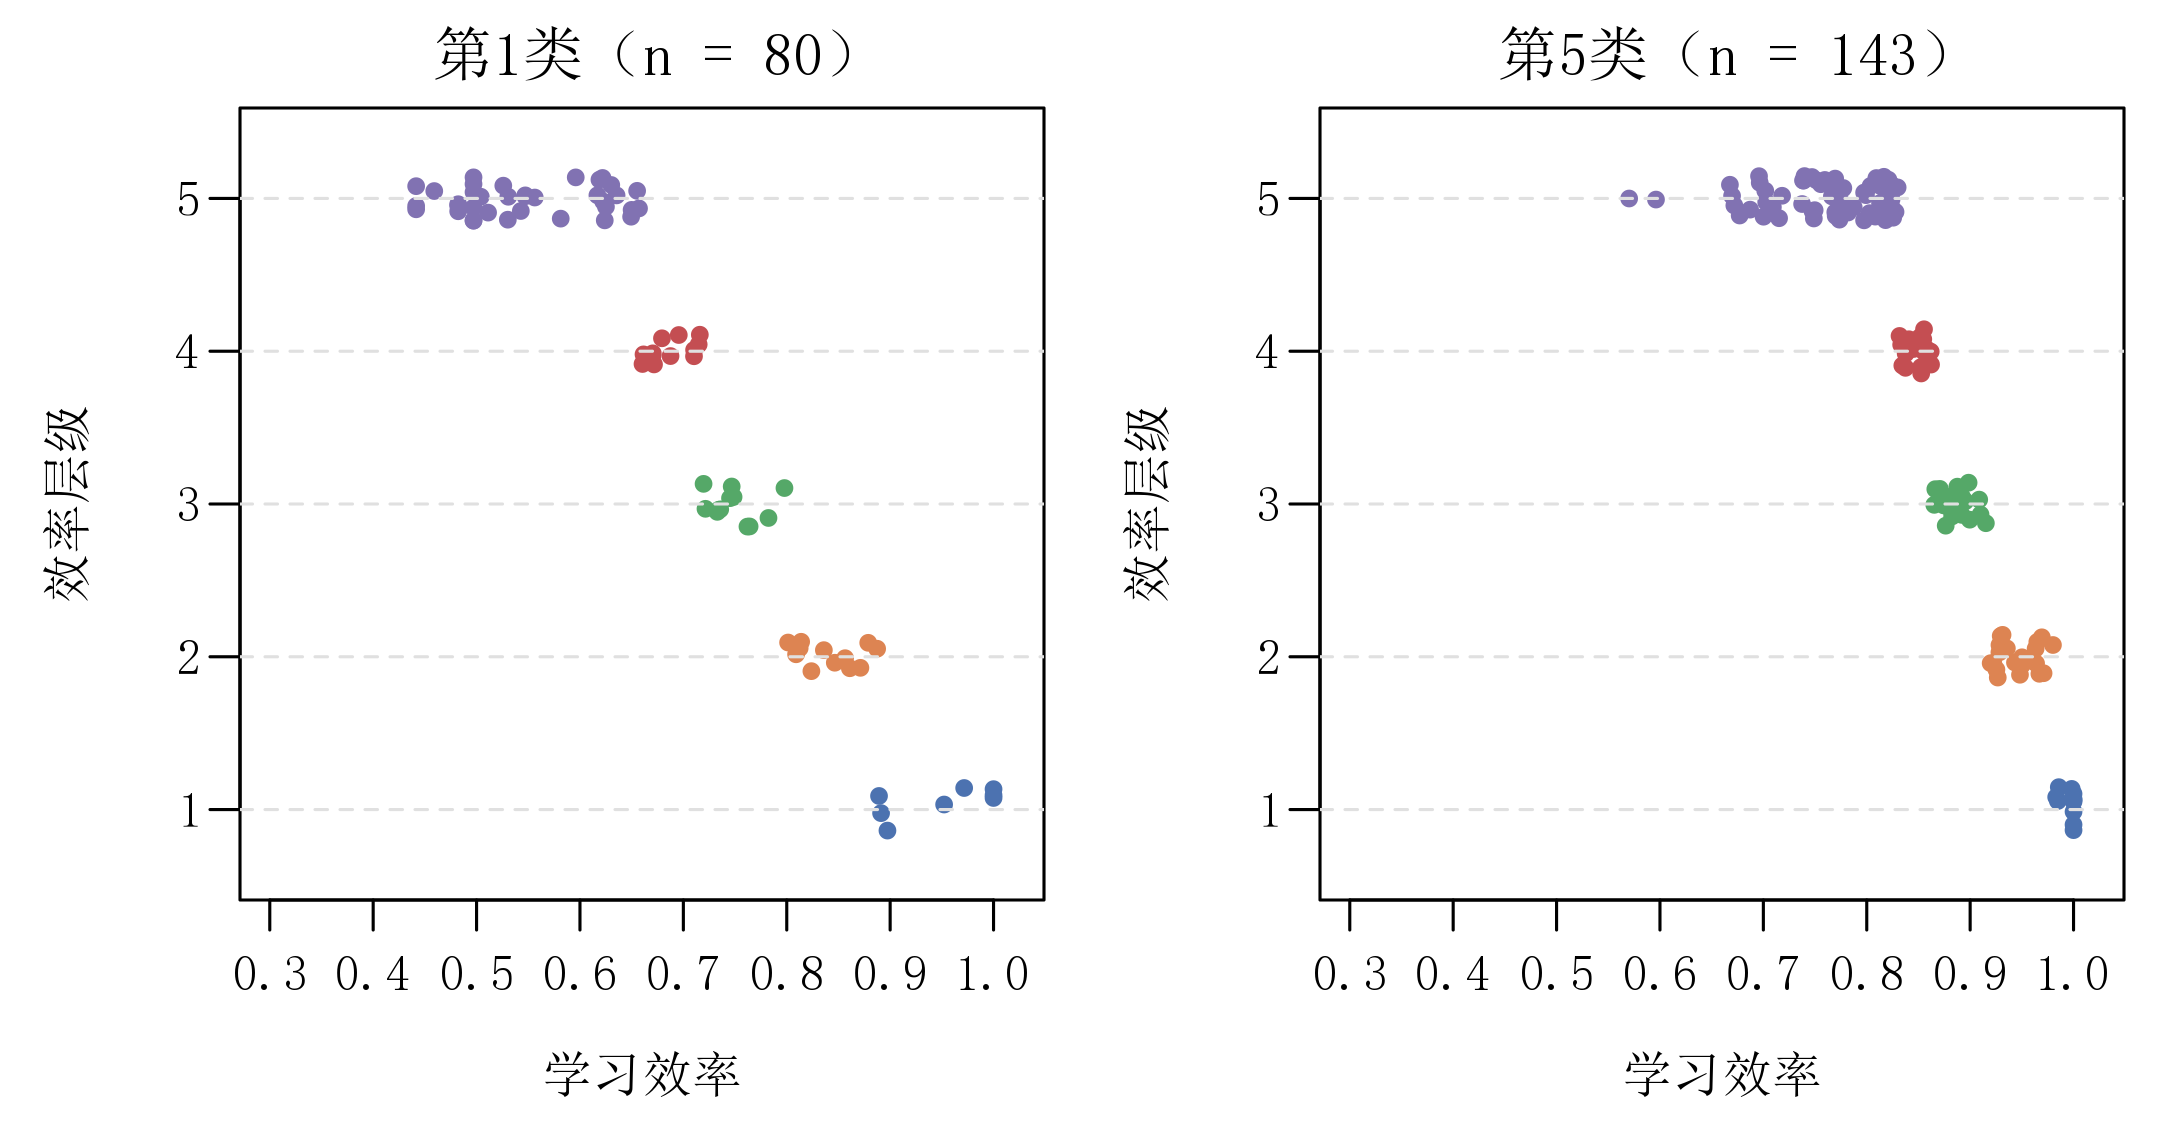
\includegraphics[width=0.95\textwidth]{fig_layer}
\caption{第 1 类与第 5 类的分层散点（横轴效率、纵轴层号；颜色区分层级）}
\label{fig:layer}
\end{figure}

\subsubsection{三准则与参考路径}

在分位带口径下计算式\eqref{eq:omega}—\eqref{eq:H}，得到 $\Omega$ 均值
1.34（范围 0.82—2.31）、$P$ 均值 0.90（0.65—1.00）、$D$ 均值 22.56
（0.67—59.94）、$H$ 均值 1.78（1.51—1.97）。$\Omega$ 普遍大于 1，说明大
多数个体相对“上层前沿”仍有产出扩张空间；$P$ 普遍小于 1，说明相对“下层前
沿”已经领先。这两个方向相反的信号同时存在，恰好对应“上不去也下不来”的
中间状态。

第 5 类第 4 层的 22 名个体见表 \ref{tab:l4}。它们的效率集中在
0.832—0.862，$\Omega$ 在 1.160—1.202，$P$ 在 0.818—0.988，$D$ 从 4.22 到
36.23，$H$ 在 1.673—1.825。按 $H$ 升序排列后，S477（$H=1.673$）排在首位，
这正是后文路径的下一站。

\begin{table}[H]
\centering
\tabfont
\caption{第 5 类第 4 层 22 名个体的三准则（按 $H$ 升序）}
\label{tab:l4}
\begin{tabular}{@{}lcccccc@{}}
\toprule
编号 & 效率 $\theta$ & $\Omega$ & $P$ & $D$ & $H$ \\
\midrule
S477 & 0.8553 & 1.1692 & 0.8178 & 16.71 & 1.6731 \\
S428 & 0.8514 & 1.1746 & 0.8307 & 15.89 & 1.6821 \\
S504 & 0.8333 & 1.2001 & 0.8587 & 15.17 & 1.6920 \\
S505 & 0.8317 & 1.2023 & 0.9486 & 11.87 & 1.7803 \\
S475 & 0.8547 & 1.1700 & 0.9384 & 11.92 & 1.7930 \\
S499 & 0.8554 & 1.1691 & 0.9408 & 16.68 & 1.7962 \\
S484 & 0.8524 & 1.1731 & 0.9440 & 21.99 & 1.7965 \\
S395 & 0.8375 & 1.1941 & 0.9612 & 16.81 & 1.7987 \\
S425 & 0.8376 & 1.1938 & 0.9610 & 18.06 & 1.7987 \\
S458 & 0.8527 & 1.1728 & 0.9460 & 17.14 & 1.7987 \\
S432 & 0.8453 & 1.1830 & 0.9573 & 22.09 & 1.8026 \\
S424 & 0.8619 & 1.1603 & 0.9409 & 10.76 & 1.8027 \\
S431 & 0.8584 & 1.1650 & 0.9444 & 10.16 & 1.8027 \\
S463 & 0.8614 & 1.1610 & 0.9415 & 5.68 & 1.8028 \\
S491 & 0.8344 & 1.1985 & 0.9716 & 4.22 & 1.8060 \\
S423 & 0.8557 & 1.1687 & 0.9517 & 11.62 & 1.8074 \\
S385 & 0.8395 & 1.1912 & 0.9686 & 6.37 & 1.8081 \\
S422 & 0.8622 & 1.1598 & 0.9494 & 13.75 & 1.8116 \\
S503 & 0.8513 & 1.1746 & 0.9621 & 36.23 & 1.8134 \\
S454 & 0.8465 & 1.1813 & 0.9686 & 9.28 & 1.8151 \\
S517 & 0.8408 & 1.1894 & 0.9787 & 25.06 & 1.8195 \\
S405 & 0.8374 & 1.1941 & 0.9879 & 11.00 & 1.8253 \\
\bottomrule
\end{tabular}
\end{table}

以 S480 为起点按 $(H,D)$ 字典序拼接路径，得到
\begin{equation}
\text{S480}\ \longrightarrow\ \text{S477}\ \longrightarrow\
\text{S456}\ \longrightarrow\ \text{S494}\ \longrightarrow\ \text{S293},
\label{eq:path}
\end{equation}
效率依次为 0.6771、0.8553、0.8806、0.9633、1.0000，单步增幅为
$+26.31\%$、$+2.96\%$、$+9.40\%$、$+3.81\%$，累计 $+47.69\%$。原文给出的
路径是 S480$\to$S502$\to$S216$\to$S18，单步 25.38\%、累计 43.97\%。两条
路径的中间站不同（因为数据是重建的），但\textbf{起点相同、方向相同、单步
增幅的头部量级几乎相同（26.31\% 对 25.38\%）、累计增幅相差 3.7 个百分点}。
在数据不可得的条件下，这已经是较强的同构证据。

值得注意的是路径的形状：第一步跨了 26.31\%，后三步合计只增加 16.9\%。这
说明“从底层跃到中层”的边际收益最大，“从中层到顶层”的边际收益迅速递减。
这一非线性结构在原文中没有被讨论，但对策略设计至关重要——它意味着\textbf{
最该做的干预是“先跳出去”，而不是“追求满分”}。

\subsubsection{复现结果与原文的逐项对照}

表 \ref{tab:repro} 把可比的项目逐条列出。总体判断是：\textbf{结构层面对
得上，数值层面部分对得上}。样本量、类型数、第 5 类人数、S480 的起始层与
效率、单步增幅五项完全或几乎完全一致；效率均值、最小值、效率—成绩相关、
第 4 层人数与效率跨度四项存在系统性偏差，偏差来源已在各小节说明。

\begin{table}[htbp]
\centering
\tabfont
\caption{复现结果与原文的锚点对照}
\label{tab:repro}
\begin{tabular}{@{}lllll@{}}
\toprule
项目 & 原文 & 本文复现 & 判定 \\
\midrule
样本量 & 519 & 519 & 一致（锚点） \\
学生类型数 & 5 & 5 & 一致（锚点） \\
第 5 类人数 & 最多 & 143/519（27.6\%） & 一致（锚点） \\
聚类轮廓宽度 & 未报告 & 0.4074（$k=5$） & 补充 \\
效率均值 & 约 0.85 & 0.7935 & 偏低 \\
效率最小值 & 约 0.50 & 0.4324 & 偏低 \\
效率—成绩相关 & 约 0.87 & 0.675 & 偏低（口径差异） \\
第 5 类第 4 层人数 & 9 & 22 & 口径差异 \\
S480 类内效率 & 0.6771 & 0.6771 & 一致（锚点） \\
S480 起始层级 & 第 5 层 & 第 5 层 & 一致（锚点） \\
S480 单步提升 & 25.38\% & 26.31\% & 相差 0.93 个百分点 \\
S480 累计提升 & 43.97\% & 47.69\% & 相差 3.72 个百分点 \\
\bottomrule
\end{tabular}
\end{table}

偏差的机制可以归纳为三条。\textbf{其一，效率水平整体偏低}，因为重建数据
在投入端保留了较大的离散性（第 1 类的 $x_1$ 低至 12.2，第 5 类高至 96.4），
而产出端被式\eqref{eq:scoregen} 压缩在 30—99，前沿个体的“产出—投入比”
没有原文那么夸张；均值下移约 0.06 属于这一机制的必然结果。\textbf{其二，
相关偏低}，因为类内评价消除了组间差异（已在上文说明）。\textbf{其三，第 4
层人数与效率跨度不同}，因为原文用剔除式、本文用分位带；若改用剔除式，第 5
类第 4 层为 20 人、效率区间 $[0.825,0.910]$，与原文的 9 人、$[0.505,
0.849]$ 更接近，但仍不等——这说明原文的表 3 可能只报告了该层的部分个体。

\subsubsection{口径敏感性讨论}
\label{sec:sens}

复现过程中有四类口径会改变结果，本文逐一给出处置与影响判断，而不把它们
埋在附录里。

\textbf{（1）聚类数。}轮廓系数显示 $k=4$ 优于 $k=5$（0.4296 对
0.4074）。若取 $k=4$，五类画像会被合并为四类，第 5 类的“高效自主”将与第
4 类的“高投入”部分混同，S480 仍会落在最差层，但路径的第二站可能改变。这
一敏感性说明：\textbf{“5 类”是原文的设定，不是数据的必然}，任何基于类型
数的结论都应附带这一说明。

\textbf{（2）层级口径。}分位带与剔除式的层号不同，但两者对 S480 的判定
一致（第 5 层）且路径首站一致（S477）。差别主要在第 4 层的规模与效率跨度
上（22 人对 20 人、跨度 0.030 对 0.085）。本文以分位带为主口径，正是因为
它能让状态空间占满；若读者更认同原文的剔除式，第 4 节的时间尺度会略有变
化，但结论方向不变。

\textbf{（3）量化细节。}时长题是否作 $\log(1+t)$ 压缩，会改变少数高投入
个体的位次，从而改变前沿的构成。本文对所有变量统一到 0—100 的秩标度，使
得这一敏感性的影响被限制在“个体位次的小幅交换”层面，不会改变类的画像。

\textbf{（4）$\varepsilon$ 与并列规则。}$\varepsilon$ 只影响“弱有效”与
“强有效”的区分，本文取 $10^{-9}$，小于任一可行松弛的量级，故不改变
$\theta$ 的数值；路径拼接的并列情形用 $(H,D)$ 字典序与“编号小者优先”两种
规则处置，由于 $H$ 在各层内呈明显梯度，并列对路径的影响可以忽略。这两项的
敏感性可以忽略。
